\chapter{Unparse Algorithmus}
\section{Verlorengehende Informationen}

Um zu verstehen was für Informationen verloren werden und der Unparser wiederherstellen muss, betrachten wir im folgenden den Parser Algorithmus von Viegener~\cite{Viegener21}. Der Algorithmus überführt einen textbasierten Diff in einen Variation-Diff um. Ein Variation-Diff ist ein gerichteter azyklischer Graph. Dieser Graph stellt dabei zeilenbasiert den textbasierten Diff dar. Die Knoten des Graphen werden durch einen Diff-Typ und einen Code-Typ eingeordnet. Diese Informationen werden der Zeil entnommen, die der Knoten repräsentiert und gelten damit auf für Zeilen eines textbasierten Diffs. Der Diff-Type kann die Werte add, remove oder none einnehmen. Add bedeutet das diese Zeile dem textbasierten Diff hinzugefügt wurde, remove das diese Zeile entfernt wurde und none das die Zeile unverändert geblieben ist. Der Code-Typ kann die Werte if, elif, else, code, oder endif haben. Dabei gibt der Code-Type an, das bei dem Wert if die Zeile eine Anweisung des if-Blocks, dass können die Präprozessor Anweisungen \#if, \#ifdef, oder \#ifndef sein, enthält und der Knoten darstellt. Bei den Wert elif es ist die Anweisung \#elif, bei else die Anweisung \#else. Bei dem Wert code des Code-Typs enthält die Zeile Code und der Knoten stellt dies dar. Der Wert endif gibt and das die Zeile die Anweisung \#endif enthält, in dem Variation-Diff ist dieser Code-Typ nicht enthalten. Die Knoten des Variation-Diffs haben höchstens zwei Elternknoten. Es gibt einen befor Elternknoten, das ist der Elternknoten, welchen der Knoten vor der Änderung hatte. Dieser Elternknoten gibt den umgebenden Präprozessor-Block vor der Änderung an. Es gibt noch einen after Elternknoten das ist der Elternknoten, welchen der Knoten nach der Änderung hat. Dieser Elternknoten gibt den umgebenden Präprozessor-Block nach der Änderung an. Nur Knoten mit Diff-Typ none haben zwei Elternknoten. Die Knoten mit dem Diff-Typ remove haben nur den befor Elternknoten und die Knoten mit dem Diff-Typ add haben nur after Elternknoten. Dabei kann ein befor Elternknoten nicht den Diff-Typ add haben und ein after Elternknoten nicht den Diff-Typ remove. Der Variation-Diff hat noch einen Knoten welcher keine widerspiegelung in dem textbasierten Diff enthält, das ist der Wurzelknoten. Der Wurzelknoten repräsentiert den ganzen textbasierten Diff. Er hat als einziger Knoten in dem Variation-Diff kein Elternknoten. Der Wurzelknoten hat immer den Diff-Typ none und den Code-Typ if, dabei ist das Feature-Mapping wahr.



\begin{algorithm}[H]
	\SetAlgoLined
	\DontPrintSemicolon
	\KwData{ein textbasierter Diff}
	\KwResult{ein Variation-Diff}
	initialisiere ein Stack/Keller $before$ mit dem Wurzelknoten\;
	initialisiere ein Stack/Keller $after$ mit dem Wurzelknoten\;
	\;
	\ForEach{Zeile in dem Patch/Diff}{
		$\delta$ $\leftarrow$ identifiziere Diff-Typ\;
		$\gamma$ $\leftarrow$ identifiziere Code-Typ\;
		$\sigma$ $\leftarrow$ gib relevante Stacks mithilfe von $\delta$ an\;
		\;
		\eIf{$\gamma$ = endif}{
			entpacke $\sigma$ bis ein Knoten mit $\gamma$ = if entpackt wurde\;
		}{
			erstelle einen neuen Knoten mit $\delta$, $\gamma$ und Eltern aus $\sigma$\;
			\If{$\gamma$ $\neq$ code}{
				füge den neuen Knoten $\sigma$ hinzu\;
			}
		}
	}
	\caption{Erstellung eines Variation-Diffs aus einem Patch}
\end{algorithm}
Der Algorithmus arbeitet wie folgt, ganz am Anfang werden zwei Stacks erstellt und jeweils mit dem Wurzelknoten initialisiert, was in Zeilen 1 und 2 des Algorithmus 1 zu sehen ist. In Zeile 4 ist eine Schleife zu sehen, welche über alle Zeilen des textbasierten Diffs geht. Dabei wird für jede Zeile zuerst der Diff-Typ $\delta$ in Zeile 5 und dann der Code-Typ $\gamma$ in Zeile 6 festgelegt. In Zeile 7 werden die relevanten Stacks $\sigma$ anhand von Diff-Typ $\delta$ bestimmt und zwar wie folgt:
\[ \sigma =
\begin{cases}
	\text{Stack } after      &, \quad \delta = \text{add}\\
	\text{Stack } befor  &, \quad \delta = \text{remove}\\
	\text{Stacks } befor \text{ und } after &, \quad \delta = \text{none}
\end{cases}
\]
Danach in Zeile 9 kommen wir zu einer if-Abfrage. Wenn der Code-Typ der bearbeiteten Zeile endif entspricht, dann wird aus den relevanten Stacks in $\sigma$ solange Knoten entnommen bis man ein Knoten mit dem Code-Type $\gamma$ if entnommen hat. In Fall das beide Stacks relevant sind, muss der if Knoten in beiden Stacks gefunden werden. Wenn der Code-Typ nicht endif entspricht kommen wir in dem else-Teil ab Zeile 11 des Algorithmus 1. Dort wird zuerst ein neuer Knoten erstellt, welcher unter anderem auch Diff-Typ $\delta$, Code-Typ $\gamma$ und Elternknoten aus den Stacks von $\sigma$ enthält. Als nächstes wird in Zeile 13 Überprüft ob der erstellter Knoten nicht von Code-Typ code ist, also den Code-Type if, elif, oder else hat. Den Code-Typ endif kann dieser Knoten nicht haben, wegen der if-Abfrage in Zeile 9, welche nicht zulässt das ein Knoten mit diesem Typ zu dieser Stelle gelangen kann. Wenn der Knoten nicht von Code-Typ code ist, dann wird dieser Knoten den relevanten Stacks aus $\sigma$ hinzugefügt, sonst wenn der Knoten den Code-Type code hat wird nichts gemacht.\\


Der vorgestellter Algorithmus ist für das Parsen von textbasierten Diffs zu Variation-Diffs ausgelegt aber es ist auch möglich den zum Parsen von C-Präprozessor-Annotierten Code zu Variation-Tree zu verwenden. Um das anstellen zu können müssen wir zwei Sachen anstellen. Zuerst wäre da die Anpassung der Eingabe, da wir C-Präprozessor-Annotierten Code haben aber der Algorithmus einen textbasierten Diff erwartet. Die zweite Sache wäre die Anpassung der Ausgabe, die Ausgabe des Algorithmus ist ein Variation-Diff, wir brauchen aber ein Variation-Tree. Um die Eingabe gerecht für den Algorithmus zu machen, müssen wir unseren C-Präprozessor-Annotierten Code in ein textbasiertes Diff verwandeln. Dazu bilden wir ein Diff mit unseren C-Präprozessor-Annotierten Code als davor und danach Zustand und bekommen ein textbasiertes Diff wo alle Zeilen gleich dem C-Präprozessor-Annotierten Code sind. Dabei hat jede Zeile dieses Diffs den Diff-Typ none. Da jetzt ein Diff gegeben ist, konnen wir auf den Diff den Algorithmus anwenden. Die Ausgabe ist dann ein Variation-Diff und der muss in eine Variation-Tree umgewandelt werden. Um dies anzustellen, bilden wir eine Projektion des Variation-Diffs auf den davor bzw. danach Zustand und bekommen ein Variation-Tree, was auch gewollt ist. Mit den gezeigten zwischen Schritten lässt sich dieser Algorithmus auch für das Parsen von C-Präprozessor-Annotierten Code zu Variation-Trees verwenden.\\


Wir wollen die Arbeitsweise des Algorithmus veranschaulichen. Dazu wenden wir den Algorithmus auf den untenstehende künstlich generierte C-Präprozessor-Annotation anwenden. Da hier eine C-Präprozessor-Annotation gegeben ist aber wir ein textbasiertes Diff brauchen, wird wie in dem Abschnitt davor vorgegangen und diese C-Präprozessor-Annotation bildet ein Diff mit sich selbst, somit ist die nötige Eingabe gegeben.
\begin{figure}[h]
\begin{itemize}
	\item[1 ] Anweisung1	(a1)
	\item[2 ] \textbf{\#if} Bedingung1 (b1)
	\item[3 ] \hspace*{0.5cm} \textbf{\#if} Bedingung2 (b2)
	\item[4 ] \hspace*{1cm}Anweisung2 (a2)
	\item[5 ] \hspace*{0.5cm}\textbf{\#else}
	\item[6 ] \hspace*{1cm}Anweisung3 (a3)
	\item[7 ] \hspace*{0.5cm}\textbf{\#endif}
	\item[8 ] \hspace*{0.5cm}Anweisung4 (a4)
	\item[9 ] \textbf{\#endif}
\end{itemize}
\end{figure}
Am Anfang des Algorithmus werden die Stacks erstellt und mit dem Wurzelknoten  initialisiert. Wir betrachten jetzt die Schleife, die über alle Zeilen des obigen Diffs geht. Wir kommen zur Zeile 1 der C-Präprozessor-Annotation, dort befindet sich eine normale Codezeile, welche nicht zur C-Präprozessor-Annotation gehört. Das ergibt das diese Zeile den Code-Typ code hat und den Diff-Typ none. Alle anderen Zeilen haben auch den Diff-Typ none, aus dem Grund wie dieser Diff gebildet wurde und deshalb lassen wir die Erwähnung des Diff-Typ für jede Zeile sein. Dasselbe gilt auch für die relevanten Stacks in $\sigma$, da alle Zeilen den Diff-Typ none haben, gilt für alle Zeilen auch die gleichen relevanten Stacks und das sind beide. Da diese Zeile nicht Code-Typ endif hat wird ein Knoten mit Code-Type, Diff-Typ, Elternknoten aus den Stacks und dem Inhalt der Zeile und den Variation-Diff hinzugefügt, wie das Aussieht ist in Abbildung 3.1 in dem Kasten nach Z.1 zu sehen. In Abbildung 3.1 beim Kasten Nach Z.2 ist der Variation-Diff nach der Bearbeitung der Zeile 2 zu sehen. Es wurde ein neuer Knoten erstellt, welcher eine if-Anweisung enthält. Die Schleife wurde fast gleich mit dem vorherigen Fall durchgelaufen, außer an der letzten if-Abfrade. Diese Abfrage was in Fall von Zeile 1 false in diesem Fall, da wir keinen Code-Typ code haben, wird diese Abfrage ausgeführt und der neu erstellter Knoten den Stacks hinzugefügt. Der nächste Kasten rechts zeigt den Variation-Diff nach Zeile 3. Der Algorithmus ist genauso wie in vorherigen Fall vorgegangen. Weiter Voran wird dem Variation-Diff im nächsten Schritt ein Code-Knoten hinzugefügt, da für die Erstellung dieses Knotens der Code selbst irrelevant ist, wurde hier genauso vorgegangen wie bei dem erstellen eines Code-Knotens in Zeile 1. In der Zeile 5 ist \#else als Anweisung gegeben. Diese Zeile hat den Code-Typ else und somit auch kein endif. Es wird in den else-Zweig der ersten Abfrage gegangen. Dort wird ein neuer Knoten mit Inhalt dieser Zeile erstellt. Der Knoten wird den Stacks hinzugefügt, da der Knoten else  als Code-Typ hat und nicht code, was die innere Abfrage erfühlt (Abb. 3.1 Nach Z.5). In der Nächsten Zeile ist wieder eine Codezeile vorhanden und aus der wird ein Code-Knoten erstellt. Wie es danach aussieht ist in Abbildung 3.1 Nach Z.6 zu sehen. Danach in der Zeile 7 treffen wir das erste mal auf die Anweisung \#endif, welche den Code-Typ endif hat. Damit gelangen wir in den if-Teil der ersten Abfrage. Den Algorithmus nach muss man aus den Stacks die Knoten solange entnehmen bis ein if Knoten kommt. Dabei werden aus den Stacks die Knoten mit else und if b2 entnommen und übrig bleiben der if b1 Knoten und der Wurzelknoten. Dieser Schritt verändert den Variation-Diff nicht. Im nächsten Schritt treffen wir wieder auf eine Codezeile und erstellen ein Knoten mit der und fügen den dem Variation-Diff hinzu, welcher in Abbildung 3.1 Nach Z.8 zu sehen ist. In der Zeile 9 ist wieder ein \#endif und wir müssen wieder Knoten aus den Stacks entnehmen. Dieses mal wird der Knoten if b1 entnommen und es bleibt nur der Wurzelknoten übrig. Damit wäre die Arbeit des Algorithmus zu Ende und wir haben als Rückgabewert einen Variation-Diff erhalten. Da aber wir einen Variation-Tree brauchen müssen wir noch eine Projektion auf den Zustand davor oder danach bilden. Danach erhalten wir ein Variation-Tree, welches genauso Aufgebaut ist, wie der Variation-Diff aus der Abbildung 3.1 Kasten Nach Z.8.
\begin{figure}[H]
\begin{tikzpicture}
\node (A) at (-0.7,0) {\fbox {
\begin{tikzpicture}
	\node[draw,diamond,fill=lightgray,thick] {root}
	child {node[draw,circle,thick] {a1}};
\end{tikzpicture}
}
};
\node (B) at (3,0) {\fbox {
		\begin{tikzpicture}
			\node[draw,diamond,fill=lightgray,thick] {root}
			child {node[draw,circle,thick] {a1}}
			child {node[draw,rectangle,thick] {\textbf{if} b1} };
		\end{tikzpicture}
	}
};
\node (C) at (7,0) {\fbox {
		\begin{tikzpicture}
			\node[draw,diamond,fill=lightgray,thick] {root}
			child {node[draw,circle,thick] {a1}}
			child {node[draw,rectangle,thick] {\textbf{if} b1}
			child {node[draw,rectangle,thick] {\textbf{if} b2}}};
		\end{tikzpicture}
	}
};
\node (D) at (11,0) {\fbox {
		\begin{tikzpicture}
			\node[draw,diamond,fill=lightgray,thick] {root}
			child {node[draw,circle,thick] {a1}}
			child {node[draw,rectangle,thick] {\textbf{if} b1}
				child {node[draw,rectangle,thick] {\textbf{if} b2}
				child { node[draw,circle,thick] {a2}}}};
		\end{tikzpicture}
	}
};
\node (E) at (0,-7) {\fbox {
		\begin{tikzpicture}
			\node[draw,diamond,fill=lightgray,thick] {root}
			child {node[draw,circle,thick] {a1}}
			child {node[draw,rectangle,thick] {\textbf{if} b1}
				child {node[draw,rectangle,thick] {\textbf{if} b2}
					child { node[draw,circle,thick] {a2}}
				}
				child { node[draw,rectangle,thick] {\textbf{else}}}
			};
		\end{tikzpicture}
	}
};
\node (F) at (5,-7) {\fbox {
		\begin{tikzpicture}
			\node[draw,diamond,fill=lightgray,thick] {root}
			child {node[draw,circle,thick] {a1}}
			child {node[draw,rectangle,thick] {\textbf{if} b1}
				child {node[draw,rectangle,thick] {\textbf{if} b2}
					child { node[draw,circle,thick] {a2}}
				}
				child { node[draw,rectangle,thick] {\textbf{else}}
					child { node[draw,circle,thick] {a3}}
				}
			};
		\end{tikzpicture}
	}
};
\node (G) at (10,-7) {\fbox {
		\begin{tikzpicture}
			\node[draw,diamond,fill=lightgray,thick] {root}
			child {node[draw,circle,thick] {a1}}
			child {node[draw,rectangle,thick] {\textbf{if} b1}
				child {node[draw,rectangle,thick] {\textbf{if} b2}
					child { node[draw,circle,thick] {a2}}
				}
				child { node[draw,rectangle,thick] {\textbf{else}}
					child { node[draw,circle,thick] {a3}}
				}
				child { node[draw,circle,thick] {a4}}
			};
		\end{tikzpicture}
	}
};
\draw[->,thick] (A) --(B);
\draw[->,thick] (B) --(C);
\draw[->,thick] (C) --(D);
\draw[thick] (D) |- (0,-3.5);
\draw[->,thick] (0,-3.5) --(E);
\draw[->,thick] (E) --(F);
\draw[->,thick] (F) --(G);
\node (a) at (-0.7,1.7) {Nach Z.1};
\node (b) at (3,1.7) {Nach Z.2};
\node (c) at (6.8,2.4) {Nach Z.3};
\node (d) at (10.8,3.2) {Nach Z.4};
\node (e) at (0,-10.3) {Nach Z.5};
\node (f) at (5.2,-10.3) {Nach Z.6};
\node (g) at (10,-10.3) {Nach Z.8};
\end{tikzpicture}
\caption{Beispiel für den Parsen Algorithmus von Viegener}
\end{figure}

 
Um weitere Informationen zu finden, die wehrend des Parse Vorgangs verloren gehen, müssen wir die Definition von Variation-Tree und Variation-Diff aus dem Schreiben Classifying Edits to Variability in Source Code~\cite{BTS+:ESECFSE22}
 betrachten. Variation-Tree wird wie folgt definiert:
 \begin{definition}
 	Ein \textsc{Variation-Tree}  $(V,E,r,\tau,l)$ ist ein Baum mit Knoten $V$ , Kanten $E \subseteq V \times V$ und Wurzelknoten $r \in V$. Jede Kante $(x,y) \in E$ verbindet einen Kinderknoten $x$ mit seinem Elternknoten $y$, bezeichnet mit $p(x) = y$. Der Knotentyp $\tau(v) \in $ \{\textsc{artifact,mapping,else}\} identifiziert einen Knoten $v \in V$ entweder als Vertreten einer Implementierungsartefakts, einer Merkmalszuordnung oder eines else-Zweig. Der Label $l(v)$ ist eine aussagenlogische Formel wenn $\tau(v) =$ \textsc{mapping}, ein Verweis auf ein Implementierungsartefakt, wenn $\tau(v) = $ \textsc{artifact}, oder leer wenn $\tau(v) =$ \textsc{else} ist. Der Wurzelknoten $r$ hat den Typ $\tau(r) =$ \textsc{mapping} und das Label $l(r) = $ \textsc{true}. Ein Knote $e$ von Typ $\tau(e) =$ \textsc{else} kann nur unterhalb eines Nichtwurzelknotens $v$ mit dem Typ $\tau(v) =$ \textsc{mapping} platziert, dabei hat ein Knoten $w$ von Typ $\tau(w) =$ \textsc{mapping} höchstens einen Knoten $u$ von dem Typ $\tau(u) =$ \textsc{else}.
 \end{definition}
  Der Variation-Diff wird dabei wie folgt definiert:
  \begin{definition}
  	Ein \textsc{Variation-Diff} ist ein gerichteter, zusammenhängender, azyklischer Graph $D=(V,E,r,\tau,l,\Delta) $, welcher einen Wurzelknoten hat, mit Knoten $V$, Kanten $E \subseteq V \times V$, Wurzelknoten $r \in V$, Knotentyp $\tau$, Knotenlabel $l$ und einer Funktion $\Delta : V \cup E \to $\{\textcolor{green}{+},\textcolor{orange}{--},\textcolor{gray}{$\circ$}\}, die definiert, ob ein Knote oder eine Kante hinzugefügt \textcolor{green}{+} wurde, entfernt \textcolor{orange}{--} wurde oder unverändert \textcolor{gray}{$\circ$} geblieben ist, so das \textsc{project}($D,t$) ein Variation-Tree für alle Zeiten $t \in \{\textcolor{green}{a},\textcolor{orange}{b}\}$ ist. Dies ist wie folgt definiert \textsc{project}$((V,E,r,\tau,l,\Delta),t) := (\{v \in V | $\textsc{exists}$(t,\Delta(v))\},\{e \in E | $\textsc{exists}$(t,\Delta(e))\},r,\tau,l)$. Dabei bedeutet \textsc{exists} für $x \in V \cup E$ folgendes, \textsc{exists}$(t,\Delta(x)) := (t = \textcolor{orange}{b} \land \Delta(x) \neq \textcolor{green}{+}) \lor (t = \textcolor{green}{a} \land \Delta(x) \neq \textcolor{orange}{-})$.
  \end{definition}
    
Aus der gegebenen Information, lässt sich herausfinden, welche Informationen währen des Parsens verlorengehen. Aus der Definition von Variation-Tree dass beim Mapping Informationen ferloren gehen. Der Informationsverlust geschieht wie folgt, die Ausgangsbedingung (z.B !A \&\& B) aus Bedingungsanweisungen (\#if !A \&\& B) in aussagenlogische Formel (z.B $\lnot$A $\land$ B) umgewandelt wird und somit die Ausgangsbedingung in Bedingungsanweisung verlorengeht. In dem Knoten des Variation-Trees ist dann die modifizierte Bedingungsanweisung (z.B.\#if $\lnot$A $\land$ B) enthalten. Die ursprüngliche Information ist dann nicht mehr in dem Variation-Tree enthalten und muss beim Unparsen wiederhergestellt werden. Für Variation-Diff verhält es sich glicht, da der Definition nach dort das mapping genauso wie in Variation-Trees verhält. Aus dem Parse-Algorithmus lässt sich entnehmen, dass die Position und die Einrückung ausgehend von Zeilenbeginn, der \#endif Anweisungen verlorengeht. Das geschieht, da der Algorithmus sich nichts zu dieser Anweisung merkt im Variation-Diff/Tree und auch keine Knoten gibt, welcher diese Anweisung darstellt. Das führt uns dazu das diese Informationen auch von uns wiedergewonnen werden müssen. Damit haben wir herausgefunden, welche Informationen während des Parsens verlorengehen und die wir wiederherstellen müssen um das Unparsen zu bewerkstelligen.



%Di.14:00 Treffen



\section{Unser Algorithmus}

%Im Baum stellen Knoten Blöcke dar, Tiefensuche geht alle blöcke eiser zweigt zuerst durch dann zum nächsten so entsteht wieder der Text



\begin{algorithm}[H]
	\SetAlgoLined
	\DontPrintSemicolon
	\KwData{ein Vatiation-Tree}
	\KwResult{ein mit C-Präprozessor-Annotierten Code}
	initialisiere einen leeren Stack/Keller $stack$\;
	initialisiere einen String $ergebniss$
	$root$ $\leftarrow$ Variation-Tree gibt Wurzelknoten aus\;
	$kinder$ $\leftarrow$ $root$ gibt seine Kinderknoten aus\;
	\For{i = n $\to$ 1 }{
		lege den Knoten aus $kinder$[i] auf den Stack $stack$\;
	}
	\While{$stack$ nicht leer ist}{
		$knoten$ $\leftarrow$ nehme das oreste Element aus dem Stack $stack$\;
		füge die gespeicherte Zeile aus $noten$ den $ergebniss$ hinzu\;
		\If{wenn knoten nicht von Typ Artefact ist und sein letztes Kindknoten nicht von Typ else oder elif ist}{
			erstelle einen Dummyknoten welcher die endif-Anweisung beinhaltet\;
			füge diesen Knoten den Stack hinzu\;
		}
		$kinder$ $\leftarrow$ $knoten$ gibt seine Kinderknoten aus\;
		\For{i = n $\to$ 1 }{
			lege den Knoten aus $kinder$[i] auf den Stack $stack$\;
		}
	}
	\caption{Ein Variation-Tree zum mit C-Präprozessor-Annotierten Code unparsen}
\end{algorithm}

\begin{tikzpicture}
	\node[draw,rectangle split,rectangle split parts=2] (A) at (0,0) {
			\begin{tikzpicture}
				\node[draw,diamond,fill=lightgray,thick] {root}
				child {node[draw,circle,thick] {a1}}
				child {node[draw,rectangle,thick] {\textbf{if} b1}
					child {node[draw,rectangle,thick] {\textbf{if} b2}
						child { node[draw,circle,thick] {a2}}
					}
					child { node[draw,rectangle,thick] {\textbf{else}}
						child { node[draw,circle,thick] {a3}}
					}
					child { node[draw,circle,thick] {a4}}
				};
				\draw [>=stealth,red,<-,line width=1mm] (1,0) -- (2,0);
			\end{tikzpicture}
	\nodepart{two} 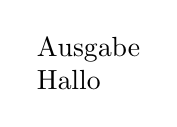
\begin{tikzpicture}
		\node[align=left] {Ausgabe \\ Hallo};
		\end{tikzpicture}};
\end{tikzpicture}


\section{Laufzeitanalyse}
\subsection{Laufzeitanalyse für Unparsen von Variation-Trees}

\subsection{Laufzeitanalyse für Unparsen von Variation-Diffs}








